\chapter{Background}
\section{Reinforcement Learning}

Reinforcement Learning (RL) is a paradigm in which an agent learns to make decisions by interacting with its environment. In the RL framework, the environment is often modeled as a Markov decision process (MDP), characterized by key components:

\begin{itemize}
  \item $S$ – the state space,
  \item $A$ – the action space,
  \item $P(s_t, a, s_{t+1})$ – the transition function, mapping from state $s_t$ and action $a$ to the next state $s_{t+1}$ with probabilities in the range [0, 1],
  \item $R(s, a)$ – the reward function, which assigns a real-valued reward to each state-action pair,
  \item $\gamma$ – the discount factor, controlling the trade-off between immediate and future rewards.
\end{itemize}

The RL agent operates based on a policy $\pi$, which maps states to actions, i.e., $\pi: S \rightarrow A$. When the agent selects an action $a_t$ in the current state $s_t$, it impacts the environment, leading to a new state $s_{t+1}$ and an immediate reward $r_t$.

\begin{figure}[htpb]
    \centering
    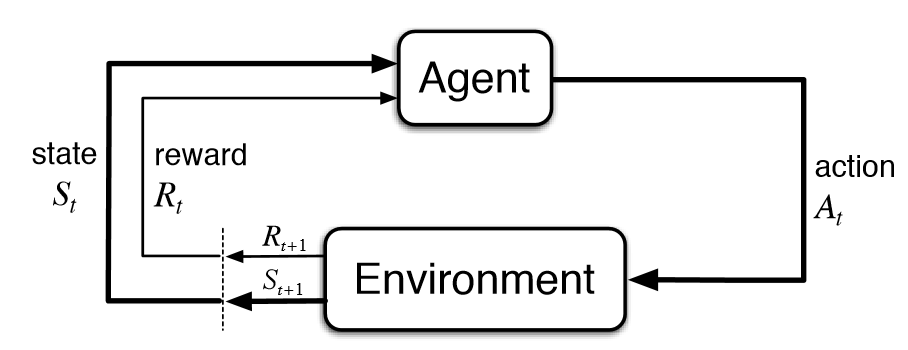
\includegraphics[scale=0.4]{images/background/RL.png}
    \centering
    \caption{Reinforcement Learning Framework}
    \label{fig:rl-framework}
\end{figure}

The primary objective of the RL agent is to maximize the expected sum of discounted rewards, denoted as $J^\pi = \sum_{t=0}^{\infty} \gamma^t r_t$. The optimal policy, denoted as $\pi^*$, is the one that maximizes this objective.

There are various approaches for training a policy using RL:

\begin{itemize}
  \item \textbf{Value-Based Approach:} This approach focuses on estimating the expected future utility from states (state value) or from action-state pairs (action value or q-value). The control policy is then directed towards actions or states that maximize the expected utility ($J^\pi$). A prominent example is the model-free deep Q-learning algorithm \cite{mnih2015human}.
  
  \item \textbf{Policy-Gradient Approach:} In this approach, a policy is defined through a parameterized differential equation, and the parameters are updated incrementally following the policy gradient. These updates aim to achieve favorable outcomes as measured by the reward function. Estimations of state or action values are often used to define these favorable outcomes. This approach is commonly referred to as an actor-critic approach.
  
  \item \textbf{Actor-Critic Approach:} Actor-critic methods combine elements of both value-based and policy-gradient approaches. An actor (policy) learns to make decisions, while a critic (value function) evaluates these decisions. A state-of-the-art example of an actor-critic algorithm is the proximal policy optimization (PPO) algorithm \cite{schulman2017proximal}.
\end{itemize}

These RL approaches provide a framework for training intelligent agents to make decisions in complex and dynamic environments, making them highly relevant to optimizing traffic signal control in urban settings.

\section{Traffic Signal Control as an MDP}

In the realm of traffic engineering, a signalized intersection represents a complex network of incoming and outgoing roads, each comprising one or more lanes. To efficiently manage traffic flow at such intersections, a set of phases, denoted as $\Phi$, is defined. Each phase, $\varphi \in \Phi$, corresponds to a specific traffic movement through the intersection, as illustrated in Figure \ref{fig:intersection-phase}. It's crucial to note that two phases are considered conflicting if they cannot be simultaneously enabled due to intersecting traffic movements.

\begin{figure}[h]
  \centering
  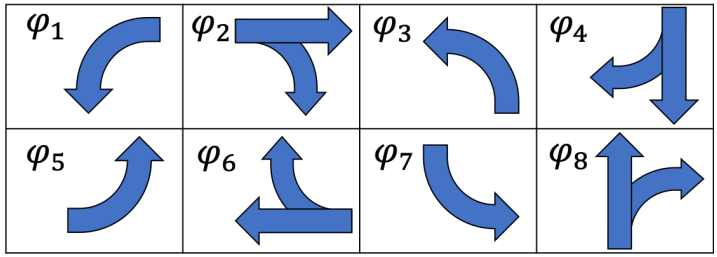
\includegraphics[width=0.6\linewidth]{images/background/intersection_phase.png}
  \caption{Example of Phases at a Signalized Intersection\cite{resco}}
  \label{fig:intersection-phase}
\end{figure}

At each discrete time step, a signal controller is tasked with selecting a combination of non-conflicting phases to enable. The objective is to optimize a long-term objective function, which may vary depending on specific goals and constraints. In the context of Reinforcement Learning (RL)-based controllers, the signalized intersection environment is commonly modeled as a Markov Decision Process (MDP), with the following components:

\begin{itemize}
  \item \textbf{State Space ($S$):} The state space encompasses the state of incoming traffic and the currently enabled phases. The definition of the state varies among studies, reflecting differing sensing capabilities. Some works assume state-of-the-art traffic sensing technologies, providing high-resolution data on incoming traffic, including information such as the number of approaching vehicles, accumulated waiting time, the number of stopped vehicles, and the average speed of approaching vehicles \cite{chen2020toward}. Others adopt less informative sensing capabilities, such as observing only the stopped queue length per lane \cite{ma2020feudal} or solely the waiting time of the first vehicle in the queue \cite{shabestary2018deep}.

  \item \textbf{Action Space ($A$):} In each time-step, the controller selects a set of non-conflicting phases to be assigned the right-of-passage (green light). If the chosen phases are different from the currently enabled ones, a mandatory yellow phase is enforced ny the system for a predefined duration. It's important to note that assigning yellow phases is not the part of the action space, it is a constraint imposed by the environment.

  \item \textbf{Transition Function ($P$):} The transition function describes the progression of traffic following the signal assignment. This progression can be defined within a simulated environment, as commonly done in research \cite{ma2020feudal}, or based on real-world traffic progression in practical implementations.

  \item \textbf{Reward Function ($R$):} The reward function serves as a critical component in RL-based signal control. Different reward functions have been proposed in the literature. Commonly used reward functions include (minus) queue length summed over all incoming lanes \cite{wiering2000multi}, (minus) total delays imposed by the intersection \cite{shabestary2018deep}, (minus) waiting time at the intersection \cite{ma2020feudal}, and (minus) traffic pressure \cite{chen2020toward}. These reward functions reflect various aspects of traffic performance and congestion alleviation.

\end{itemize}

The modeling of traffic signal control as an MDP provides a foundation for applying RL techniques to optimize signal operation, ultimately contributing to more efficient and adaptive traffic management strategies.

\section{Evaluation environments for RL-based signal controllers} \label{sec:evaluation-environments}
According to \cite{resco}, previous research in the field of traffic signal control has often relied on custom-made scenarios tailored for evaluating specific Reinforcement Learning (RL) algorithms. For instance, Jinming and Feng (2020) utilized the well-established Simulation of Urban Mobility (SUMO) environment for their experiments. SUMO enjoys widespread acceptance within the transportation community and serves as a reasonable testbed choice for such studies. However, it's worth noting that Jinming and Feng's reported scenario, based on the real-world city of Monaco, was a modified version. This modified scenario included 18 synthetic traffic signals beyond the official "Monaco SUMO Traffic (MoST)" scenario and incorporated non-validated inflated traffic demands \cite{codeca2018monaco}.

Another notable simulation testbed, CityFlow, was presented by Zhang et al.\cite{zhang2019cityflow}. However, CityFlow has two primary limitations. Firstly, unlike SUMO, CityFlow lacks rigorous calibration and evaluation within the general transportation community. Although it claims to produce equivalent output as SUMO, this claim is primarily based on results from simplified grid network scenarios. Secondly, while CityFlow offers the Manhattan, New York network as a common benchmark scenario, the support for this scenario's representation of real-world city layouts and demands is limited.

Additionally, some relevant publications have conducted evaluations using the Autonomous Intersection Management (AIM) simulator. The primary drawback of the AIM simulator lies in its lack of traffic scenarios based on real-world cities. AIM typically generates simple grid networks with symmetric intersections. While one might draw parallels between such grid networks and the road layout in Manhattan, New York, a more in-depth analysis of traffic trends is needed to substantiate such claims and their relevance to the real world \cite{pham2013learning}\cite{dresner2008multiagent}\cite{ma2020feudal}.
